%versi 2 (8-10-2016)
\chapter{Landasan Teori}
\label{chap:teori}


Pada bab ini akan berisi landasan-landasan teori yang dipakai pada penelitian ini.

\section{Code Igniter}
\label{sec:codeigniter}


CodeIgniter\cite{codeigniter3} adalah \textit{framework} untuk pembuat website yang menggunakan \textit{PHP}. \textit{CodeIgniter} mempermudah \textit{developer} untuk meminimalisir penggunaan kode untuk mengakses suatu fungsi. Seperti untuk mengambil data pada \textit{database}, mengakses file \textit{php} lainnya. Penggunaan \textit{framework CodeIgniter} juga mudah.\textit{ Developer} tidak perlu melakukan banyak konfigurasi--konfigurasi saat melakukan \textit{setup}.\textit{CodeIgniter} juga memberikan dokumentasi yang lengkap. Permasalahan \textit{routing}  sudah diselesaikan oleh \textit{framework} ini. \textit{ Framework} ini secara otomatis akan mengarah ke file dalam \textit{directory controllers} sesuai dengan \textit{path-abempty} pada \textit{URI}  dan menjalankan \textit{method} \texttt{index()}.


\begin{figure}[H]
	\centering
	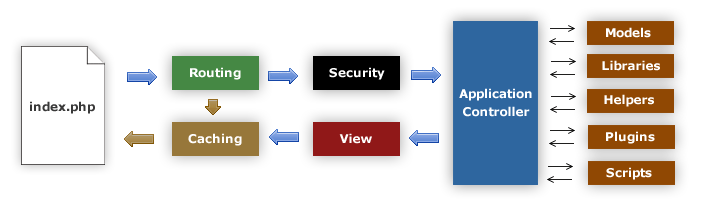
\includegraphics[scale=0.8]{mvc} 
	\caption{Flowchart MVC}
	\label{fig:appflowchart} 
\end{figure}


\textit{CodeIgniter} menerapkan arsitektur \textit{MVC} yang dapat dilihat pada gambar \ref{fig:appflowchart}, file \texttt{index.php} berfungsi mengatur routing dan mengarahkan ke \textit{application controller} yang berada di \textit{directory controller} dan melalui \textit{controller} akan dipanggil \textit{models, libraries, helpers, etc} yang dibutuhkan dengan perintah \texttt{\$this->load-><<apa\_yang\_mau\_diload>>(\lq<<nama\_file>>\rq)}. Masukan akan diolah melalui \textit{models} dan hasil yang sudah siap akan dikirim ke \textit{view} melalui \textit{controller}. Fitur tambahan dari arsitektur \textit{CodeIgniter} adalah saat \textit{router} memeriksa \textit{HTTP request} jika \textit{cache} tersedia maka akan dikirimkan \textit{cache} tersebut dan jika tidak ada \textit{cache} maka \textit{security} akan memeriksa dan melakukan filter terhadap \textit{HTTP request} seperti pada gambar \ref{fig:appflowchart}. 

\subsection{Controller}

\textit{Controller} adalah pusat dari aplikasi, \textit{controller} menangani apa yang harus dilakukan dari \textit{HTTP request}. Dalam CodeIgniter untuk menginisiasi \textit{controller} cukup menulis nama kelas diikuti dengan \texttt{extends CI\_Controller} sebagai contoh:

\begin{lstlisting}
<?php
defined('BASEPATH') OR exit('No direct script access allowed');
		
class Welcome extends CI_Controller {

	public function index()
	{
		$this->load->view('welcome_message');
	}
}
\end{lstlisting}

\textit{CodeIgniter} secara otomatis akan menjalankan \textit{method} \texttt{index()} jika tidak diperintahkan untuk menjalankan \textit{method} tertentu. Untuk menjalankan \textit{method} lain hanya perlu ditambahkan \textit{path-abempty} seperti  \texttt{example.com/index.php/Welcome/<<nama\_method>>}.
fungsi diatas akan mengembalikan file \textit{welcome\_message.php} pada direktori \textit{view}. Developer dapat menaruh parameter pada \textit{view} tersebut.

\begin{lstlisting}
<?php
defined('BASEPATH') OR exit('No direct script access allowed');
	
class Welcome extends CI_Controller {
	
	public function __construct(){
		parent::_construct();
		$this->load->database();
		$this->load->model(contoh_model);
	}
	
	public function index()
	{
		$t = "hello";
		$this->load->view('welcome_message',array(
		't' => $t));
	}
}
\end{lstlisting}


Fungsi \textit{constructor} yang dijalankan pada \textit{codeigniter} harus memanggil \texttt{parent::construct()}. Dalam contoh diatas juga dapat dilakukan \textit{load model} dan \textit{database}. File \textit{model} akan berada di direktori \textit{model} sedangkan untuk \texttt{\$this->load->database()} akan melakukan \textit{load} pada \textit{database} menggunakan parameter yang ada di direktori \texttt{/config/database.php}. Begitu juga dengan kebutuhan--kebutuhan lainnya dapat dilakukan dengan \textit{method} \texttt{\$this->load}.


\subsection{Model}

\textit{Model} berfungsi sebagai \textit{logic} dari aplikasi. \textit{ Model} pada \textit{CodeIgniter} bersifat opsional, tetapi disediakan untuk \textit{developer} yang ingin menggunakan MVC\cite{codeigniter3}. 


\begin{lstlisting}
class Blog_model extends CI_Model {
	
	public function get_last_ten_entries()
	{
		$query = $this->db->get('entries', 10);
		return $query->result();
	}
}
\end{lstlisting}

\textit{Model} pada \textit{CodeIgniter} harus diikuti dengan \texttt{extends CI\_Model}. Hal yang berurusan terhadap \textit{database} dapat dilakukan dengan perintah \texttt{\$this->db->query(\lq<<isi query>>\rq)} atau untuk mempermudah, beberapa fungsi \textit{MYSQL} dasar disediakan oleh \textit{CodeIgniter}.\textit{ Method} bisa langsung digunakan seperti \texttt{\$this->db->get(\lq<<nama tabel>>\rq)}
untuk mengambil semua nilai dari tabel tersebut. Untuk dapat mengakses \textit{database} maka harus dipasang \textit{database} yang akan digunakan pada \texttt{config/database.php}.

\begin{lstlisting}
		
$config['hostname'] = 'localhost';
$config['username'] = 'myusername';
$config['password'] = 'mypassword';
$config['database'] = 'mydatabase';
$config['dbdriver'] = 'mysqli';
$config['dbprefix'] = '';
$config['pconnect'] = FALSE;
$config['db_debug'] = TRUE;

$this->load->model('model_name', '', $config);
\end{lstlisting}

File \texttt{database.php} diatas menyimpan kredensial dari \textit{database} yang digunakan. Mulai dari \textit{hostname, username, password dll}.

\subsection{View}


\textit{View} tidak pernah dipanggil secara langsung, \textit{view} harus dipanggil melalui \textit{controller}\cite{codeigniter3}.
\textit{View} pada \textit{CodeIgniter} ditaruh pada direktori \textit{view}. Pemanggilan \textit{view} menggunakan \textit{method} 
\begin{lstlisting}
$this->load->view('nama_view');
\end{lstlisting}

Jika \textit{controller} ingin mengirimkan data kepada \textit{view} maka perlu dilakukan 

\begin{lstlisting}
$t = "hello";
$this->load->view('welcome_message',array(
't' => $t));
\end{lstlisting}

Selanjutnya untuk menampilkan data tersebut ke halaman
 
\begin{lstlisting}
<?php echo $t ?>
\end{lstlisting}

\subsection{\textit{Libraries} pada Code Igniter}
\subsubsection{Loader}
\subsubsection{Migration}
\subsubsection{Email}
\subsubsection{Input}
\subsubsection{Migrations}
\subsubsection{Session}

\section{Phpspreadsheet}
\label{section:phpspreadsheet}

PhpSpreadsheet adalah \textit{library} yang ditulis dengan bahasa PHP berguna untuk membaca dan menulis file dengan jenis spreadsheet seperti Excel dan LibreOffice Calc\cite{phpspreadsheet}. Format--format yang didukung oleh phpspreadsheet dapat dilihat pada tabel \ref{tab:phpspreadsheet supported}. Pada penelitian kali ini phpspreadsheet hanya digunakan untuk menulis ke dokumen dengan \textit{extension} \texttt{.xls}

\begin{table}[H]
	\centering
	\begin{tabular}{|p{0.5\textwidth}|c|c|}
		\hline
		\textbf{Format} & \textbf{Reading} & \textbf{Writing} \\ \hline
		Open Document Format/OASIS (.ods) & \checkmark & \checkmark \\ \hline
		Office Open XML (.xlsx) Excel 2007 and above & \checkmark & \checkmark \\ \hline
		BIFF 8 (.xls) Excel 97 and above & \checkmark & \checkmark \\ \hline
		BIFF 5 (.xls) Excel 95 & \checkmark  & \\ \hline
		SpreadsheetML (.xml) Excel 2003 & \checkmark & \\ \hline
		Gnumeric & \checkmark & \\ \hline
		HTML & \checkmark & \checkmark \\ \hline
		SYLK & \checkmark & \\ \hline
		CSV & \checkmark & \checkmark \\ \hline
		PDF (using either the TCPDF, Dompdf or mPDF libraries, which need to be installed separately) & & \checkmark \\ 
		\hline
	\end{tabular}
\caption{Tabel format yang didukung oleh phpspreadsheet}
\label{tab:phpspreadsheet supported}
\end{table}

\subsection{Kelas pada Phpspreadsheet}
Pada penelitian kali ini kelas utama yang digunakan adalah kelas \textit{Spreadsheet}. Kelas \textit{Spreadsheet} dapat diakses menggunakan \texttt{use PhpOffice$\backslash$PhpSpreadsheet$\backslash$Spreadsheet}.
 \textit{Method} yang dimiliki oleh \textit{library} \textit{PhpSpreadsheet} yang digunakan pada penelitian kali ini:

\begin{itemize}
	\item \textit{Spreadsheet} \\
	Kelas \textit{Spreadsheet} dapat diakses dengan menggunakan: 
	\begin{lstlisting}
use PhpOffice\PhpSpreadsheet\Spreadsheet;
$spreadsheet = new Spreadsheet();
	\end{lstlisting} 
	\textit{Constructor} kelas \textit{Spreadsheet} tidak menerima parameter apapun, dan \textit{return value} adalah \textit{mixed}. \textit{Method} yang tersedia pada kelas \texttt{Spreadsheet}:  
 \begin{itemize}
 	\item \textbf{\texttt{createSheet([\$sheetIndex:null|int=null])}}\\ \textit{Method} ini berfungsi untuk membuat \textit{sheet}.\\
 	\textit{Parameter}: \texttt{\$sheetIndex}, \textit{index} dari sheet dikosongkan jika menaruh sheet pada \textit{index} terakhir. \\ 
 	\textit{Return}: Kelas \texttt{Worksheet}.
 	
 	\item \textbf{\texttt{setActiveSheetIndex(\$pIndex:int)}}\\ Memilih \textit{sheet} yang ingin dijadikan \textit{active} berdasarkan \textit{index}. \\
 	\textit{Parameter}: \$pIndex, tipe data \textit{int}, \textit{index} dari \textit{Worksheet}. \\
 	\textit{Return}: Kelas \texttt{Worksheet}.
 	
 	\item \textbf{\texttt{getActiveSheet()}}\\
 	 Mengembalikan kelas \textit{Worksheet} yang aktif.\\
 	\textit{Parameter}: Tidak ada. \\ 
 	\textit{Return}: Kelas \texttt{Worksheet}.
 \end{itemize}

\item \textit{Worksheet} \\ 
Kelas \textit{Worksheet} adalah kelas yang mengatur nilai dari \textit{cell}, \textit{cell style}, judul \textit{sheet} dll. Pembuatan kelas ini dapat dilakukan dengan:
\begin{lstlisting}
$spreadsheet->createSheet();
\end{lstlisting}
Variabel \textit{\$spreadsheet} adalah kelas \texttt{Spreadsheet}, \textit{method} yang tersedia pada kelas \texttt{Worksheet}:

\begin{itemize}
	\item \textbf{\texttt{getStyle(\$pCellCoordinate:string)}}\\ 
	Mengembalikan kelas \texttt{Style}.\\
	\textit{Parameter}: \texttt{\$pCellCoordinate} koordinat dari \textit{cell} atau \textit{range}, contoh : 'A1','A1:E1'.\\
	\textit{Return}: Kelas \texttt{Style}.
	
	\item \textbf{\texttt{setCellValue(\$pCoordinate : string , \$pValue : mixed )}}\\ 
	Merubah suatu nilai pada \textit{cell} tertentu. \\ 
	\textit{Parameter}:
	\begin{itemize}
		\item \texttt{\$pCoordinate}: Koordinat dari \textit{cell} contoh: 'A1'.
		\item \texttt{\$pValue}: Nilai baru dari \textit{cell} tersebut.
	\end{itemize}
	\textit{Return}: \texttt{\$this}.
	
	\item \textbf{\texttt{mergeCells(\$pRange:string)}}\\ Melakukan \textit{merge} pada \textit{cell}. \\ 
	\textit{Parameter}: \texttt{\$pRange} \textit{cell range} yang ingin dilakukan \textit{merge}, contoh: 'A1:E1'. \\
	\textit{Return}: \texttt{\$this}.
	\item \textbf{\texttt{setTitle(\$pValue:string, \$updateFormulaCellReferences:bool = true, \$validate:bool:true)}}\\
	 Berfungsi untuk memberi judul pada \textit{sheet}. \\
	 \textit{Parameter}:
	 \begin{itemize}
	 	\item \texttt{\$pValue}: \textit{String} yang akan dijadikan nama judul.
	 	\item \texttt{\$updateFormulaCellReferences}: \textit{Flag} untuk menentukan \textit{cell reference} pada \textit{formula} akan dirubah mengikuti judul baru. Direkomendasikan untuk tidak merubah nilai variabel ini.
	 	\item \texttt{\$validate}: Nilai asal adalah \textit{true}, pasang nilai \textit{false} untuk melewati validasi dari judul baru.
	 \end{itemize}
 	\textit{Return}: \texttt{\$this}.
	\item \textbf{\texttt{getRowDimension(\$pRow:int,\$create:bool = true)}} \\ 
	Mengambil dimensi baris pada baris tertentu. \\
	\textit{Parameter}: 
	\begin{itemize}
		\item \texttt{\$pRow}: \textit{Index} dari baris.
		\item \texttt{\$create}: Nilai \textit{default} adalah \textit{true}.
	\end{itemize}
	\textit{Return}: Kelas \texttt{RowDimension}.
	\item \textbf{\texttt{getColumnDimension(\$pColumn:string, \$create : bool = true)}} \\
	Mengambil dimensi kolom pada kolom tertentu
	\textit{Parameter}:
	\begin{itemize}
		\item \texttt{\$pColumn}: String dari kolom, contoh: 'A'.
		\item \texttt{\$create}: Nilai \textit{default} adalah \textit{true}.
	\end{itemize}
	\textit{Return}: Kelas \texttt{ColumnDimension}.
\end{itemize}

\item \textit{Style} \\ 
Kelas \textit{Style} adalah kelas yang mengatur \textit{style} dari suatu \textit{cell} seperti \textit{alignment}, \textit{fill},\textit{font} dll. Kelas \textit{Style} dapat diakses menggunakan:
\begin{lstlisting}
$worksheet->getStyle('A1');
\end{lstlisting}
Variabel \textit{\$worksheet} adalah kelas \textit{Worksheet}, \textit{method} yang tersedia pada kelas \texttt{Style}:
	\begin{itemize}
		\item \textbf{\texttt{getFill()}}\\
		 Mengembalikan kelas \textit{Fill}. untuk merubah \textit{fill} pada suatu \textit{cell} dapat memanggil \texttt{setFillType()} pada kelas \textit{Fill}.	\\
		 \textit{Parameter}: Tidak ada.
		 \textit{Return}: Kelas \texttt{Fill}.
		\item \textbf{\texttt{getAlignment()}} \\
		 Mengembalikan kelas \textit{Alignment}, untuk merubah \textit{alignment} pada suatu \textit{cell} dapat memanggil \texttt{setHorizontal()} atau \texttt{setVertical()} pada kelas \textit{Alignment}. \\
		\textit{Parameter}: Tidak ada. \\
		\textit{Return}: Kelas \texttt{Alignment}.
		\item \textbf{\texttt{getFont}} \\
		 Mengembalikan kelas \textit{Font}, untuk merubah penebalan kata dapat menggunakan \texttt{setBold()} dengan masukan \textit{boolean}. \\
		\textit{Parameter}: Tidak ada. \\
		\textit{Return}: Kelas \texttt{Font}.
		
	\end{itemize}

\item \textit{Xls} \\
Kelas \texttt{Xls} memiliki 2 tipe yaitu \textit{writer} dan \textit{reader}. Pada penelitian kali ini tipe \textit{Xls} yang digunakan hanya tipe \textit{writer}. Kelas \textit{Xls} dapat diinisiasi dengan:
\begin{lstlisting}
$writer = new \PhpOffice\PhpSpreadsheet\Writer\Xls($spreadsheet);
\end{lstlisting}
\textit{Constructor} dari kelas \textit{Xls} menerima masukan berupa kelas \textit{Spreadsheet}, \textit{method} dari kelas \texttt{Xls}: \\
\textbf{\texttt{Save(\$pFilename:resource|string)}}, berfungsi untuk menyimpan \textit{Spreadsheet} menjadi \textit{file} \\
\textit{Parameter}: \texttt{\$pFilename}, menerima masukan \textit{resource} atau string. \\
\textit{Return}: \texttt{void}. 


\end{itemize} 


\subsection{Instalasi Phpspreadsheet}
Sebelum dapat menginstalasi phpspreadsheet dibutuhkan composer. Composer dapat diunduh pada \url{getcomposer.org}. 

\begin{lstlisting}
composer require phpoffice/phpspreadsheet
\end{lstlisting}

perintah tersebut digunakan untuk membuat file \texttt{composer.json} dan menginstalasi \textit{dependencies} tersebut. 

\begin{lstlisting}
<?php

require 'vendor/autoload.php';
use PhpOffice\PhpSpreadsheet\Spreadsheet;
$spreadsheet = new Spreadsheet();
\end{lstlisting}

Penggunaan phpspreadsheet secara dasar membutuhkan perintah \texttt{use PhpOffice$\backslash$Phpspread-\\sheet$\backslash$Spreadsheet} dan \texttt{new Spreadsheet()}.

\subsection{Contoh Penulisan Nilai pada \textit{cell}}

\textit{Phpspreadsheet} menyediakan suatu \textit{method} untuk dapat menaruh atau merubah \textit{value} pada cell tertentu

\begin{lstlisting}
$sheet = $spreadsheet->getActiveSheet();
$sheet->setCellValue('A1', 'PhpSpreadsheet');
\end{lstlisting}

 Fungsi diatas akan menulis \lq PhpSpreadsheet \rq pada kolom \lq A1 \rq . \textit{PhpSpreadsheet} memiliki \textit{method} untuk merubah nilai dari \textit{cell} tertentu dengan menggunakan \texttt{setCellValue('kolom','nilai')}.


\subsection{Contoh Penulisan Spreadsheet ke Xls }

\textit{Phpspreadsheet} dapat melakukan \textit{read and write} ke banyak format. Mulai dari \textit{xls,xlsx,csv} dll. Pada kali ini format yang akan digunakan adalah format  \textit{xls}.

\begin{lstlisting}
$writer = new \PhpOffice\PhpSpreadsheet\Writer\Xls($spreadsheet);
$writer->save("05featuredemo.xls");
\end{lstlisting}

Penggunaan fungsi \textit{write} dari \textit{phpspreadsheet} membutuhkan kelas \texttt{\textbackslash PhpOffice\textbackslash PhpSpread-\newline sheet\textbackslash Writer\textbackslash Xls()}. Kelas lain yang dapat digunakan untuk \textit{read}\&\textit{write} adalah \texttt{\textbackslash PhpOffice\textbackslash\\ PhpSpreadsheet\textbackslash IOFactory::createWriter(\$ spreadsheet, "Xls")}

\section{Bootstrap}
\textit{Bootstrap} adalah \textit{framework} paling terkenal untuk membuat \textit{site} yang \textit{mobile-first} dan \textit{res\-pon\-sive}\cite{bootstrap}.Dapat dilihat pada tabel \ref{tab:bootstrap mobile supported} dan tabel \ref{tab:bootstrap desktop supported}.  Hampir semua \textit{browser} pada \textit{desktop} dan \textit{mobile} dapat menjalankan \textit{bootstrap}.

\begin{table}[H]
	\centering
	\resizebox{\textwidth}{!}{
	\begin{tabular}{|l|l|l|l|l|l|}	
		\hline	
		 & \textbf{Chrome} & \textbf{Firefox} & \textbf{Safari} & \makecell[l]{\textbf{Android} \& \\ \textbf{WebView}} & \makecell[l]{\textbf{Microsoft} \\ \textbf{Edge}} \\ \hline
		\textbf{Android} & Supported & Supported & - & \makecell[l]{Android v5.0+ \\ Supported} & Supported \\ \hline
		\textbf{IOS} & Supported & Supported & Supported & - & Supported \\ \hline
		\textbf{Windows 10 Mobile} & - & - & - & - & Supported \\ \hline				
	\end{tabular}}
	\caption{\textit{Browser Mobile} yang mendukung \textit{bootstrap}}
	\label{tab:bootstrap mobile supported}
\end{table}

\begin{table}[H]
	\centering
	\resizebox{\textwidth}{!}{
		\begin{tabular}{|l|l|l|l|l|l|l|}	
			\hline	
			& \textbf{Chrome} & \textbf{Firefox}  &\makecell[l]{\textbf{Internet}\\\textbf{Explorer}} & \makecell[l]{\textbf{Microsoft}\\\textbf{Edge}} & \textbf{Opera} & \textbf{Safari} \\ 
			\hline
			\textbf{Mac} & Supported & Supported & - & Supported & Supported & Supported  \\ \hline
			\textbf{Windows} & Supported & Supported & \makecell[l]{Supported \\ IE10+} & Supported & Supported & Not supported\\ \hline		
	\end{tabular}}
	\caption{\textit{Browser Desktop} yang mendukung \textit{bootstrap}}
\label{tab:bootstrap desktop supported}
\end{table}






\subsection{Pemasangan Bootstrap}
Pemasangan dilakukan dengan cara mengunduh \textit{compiled css and jss} yang disediakan oleh \textit{bootstrap}.

\begin{lstlisting}
<head>
	<link rel = "stylesheet" href = "css/bootstrap.css">
	<script src = js/bootstrap.js></script>
</head>


\end{lstlisting}

Pemasangan \textit{bootstrap} memerlukan \textit{import} file \textit{css dan js} dari \textit{compiled bootstrap} yang telah diunduh. Cara lain yang dapat dilakukan adalah 

\subsection{Contoh Penggunaan Bootstrap}

Cara penggunaan \textit{bootstrap} adalah dengan memasukkan kelas-kelas yang disediakan oleh \textit{bootstrap}.

\begin{lstlisting}
<form>
	<div class="form-group">
		<label>Email address</label>
		<input type="email" class="form-control"
			placeholder="Enter email">
	</div>
	<div class="form-group">
		<label>Password</label>
		<input type="password" class="form-control">
	</div>
	<div class="form-check">
		<input type="checkbox" class="form-check-input">
		<label class="form-check-label">Check me out</label>
	</div>
	<button type="submit" class="btn btn-primary">Submit</button>
</form>
\end{lstlisting} 

Sebagai contoh akan dilakukan pembuatan form menggunakan \textit{bootstrap}. \texttt{<input>, <select>, <textarea>} menggunakan \textit{class form--control}, kelas tersebut sudah mengatur \textit{style} untuk \textit{focus state}, ukuran, dan tampilan umum. Sedangkan \textit{class form--group} untuk mengatur struktur dari form\cite{bootstrap}.



 
